\documentclass[a4paper,12pt]{article}

% don't forget the document class, generally : \documentclass[a4paper,12pt]{article}

\usepackage[utf8]{inputenc}
\usepackage[french]{babel}
\usepackage{graphicx}
\usepackage{gensymb}
\usepackage{amsmath}
\usepackage{float}
\usepackage{scrextend}
\usepackage{caption} 
\usepackage{siunitx}
\usepackage{enumitem}
\usepackage{amsthm}
\usepackage{fancyhdr}
\usepackage{amssymb}
\usepackage{wrapfig}
\usepackage{geometry}
\usepackage{standalone}
\usepackage{import}
\usepackage[usenames, dvipsnames]{color}

 \usepackage{biblatex} % manages bibliography and references
\addbibresource{sample.bib}


\geometry{hmargin=1in, vmargin=1in}

 \newenvironment{absolutelynopagebreak}
 {\par\nobreak\vfil\penalty0\vfilneg
 \vtop\bgroup}
 {\par\xdef\tpd{\the\prevdepth}\egroup
 \prevdepth=\tpd}
 
 \pagestyle{fancy}                        
\fancyhf{}                               
\fancyhf[HL]{Application des maths}                
\fancyhf[HR]{Géométrie euclidienne}             
\fancyhf[FC]{\thepage/\pageref{Lastpage}}
 
\newtheorem{definition}{Définition}[section]
\newtheorem{theorem}{Théorème}
\newtheorem{corollary}{Corollaire}[theorem]
\newtheorem{lemma}[theorem]{Lemme}
\newtheorem*{hyp}{Hypothèse}
\newtheorem*{concl}{Conclusion}
\newtheorem*{remark}{Remarque}

\captionsetup{format=default,labelformat=simple,labelsep=colon,
justification=justified,font={sf,small},labelfont=bf,
textfont=default} 



\begin{document}

\pagebreak
\subsubsection{Théorème 2}
\begin{theorem}\label{semblableTh2}
Si deux paires de parallèles découpent sur une sécante deux segment isométriques, elles le font sur toute autre sécante.
\end{theorem}

\begin{proof}
Nous considérons la droite $m$ qui a $m'$ comme sécante et deux paires de parallèles ($a$, $b$, $c$ et $d$) qui interceptent m et m' en huits point (respectivement $A$, $B$, $C$, $D$, $A'$, $B'$, $C'$, et $B'$). Nous construisons les parallèles de sorte à ce que $AB \equiv CD$.

\begin{figure}[H]
        \centering
        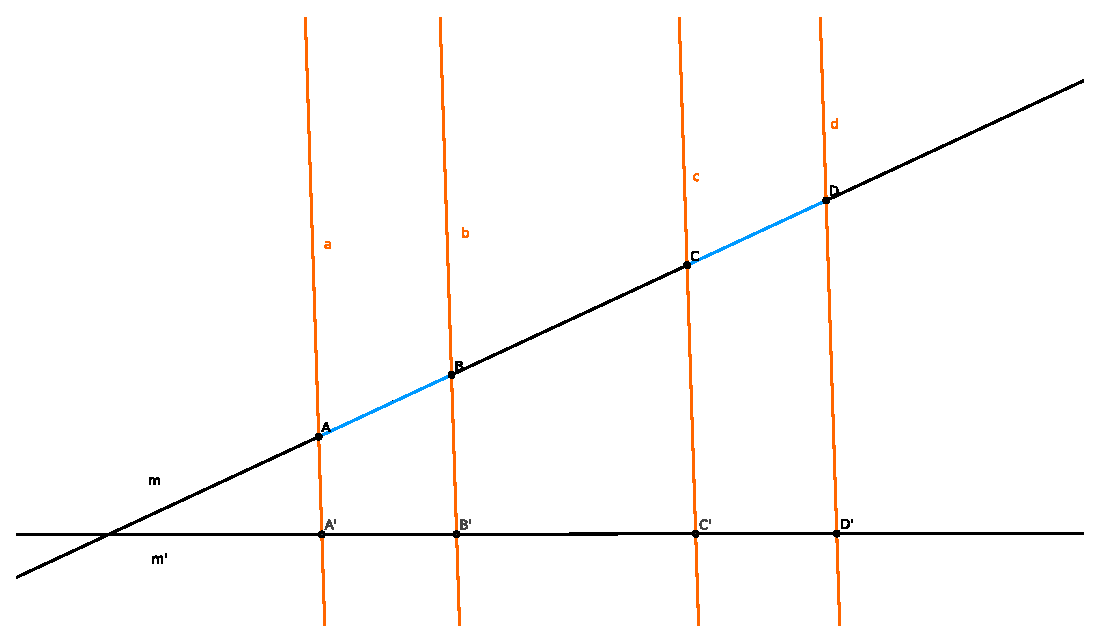
\includegraphics[scale=0.2]{semblable2.1.eps}
    \end{figure}

\begin{hyp}
\begin{itemize}
    \item $m \cap m'$
    \item a, b c et d sont parallèles
    \item $AB \equiv CD$
\end{itemize}
\end{hyp}
\begin{concl}
$A'B' \equiv C'D'$
\end{concl}
Nous construisons deux droites $e$ et $f$ qui passent respectivement par $A$ et $D$ et sont parallèles à $m'$.\\
Nous nommons $E = e \cap b$ et $F = f \cap c$.\\
Grâce au théorème de la transversale, nous savons que $\angle ABE \equiv \angle FCD$ et $\angle BAE \equiv \angle FDC$. Nous pouvons en déduire que $\triangle ABE$ et $\triangle FCD$ sont isométriques ($2^{me}$ cas d'isométrie des triangles).\\
\begin{figure}[H]
        \centering
        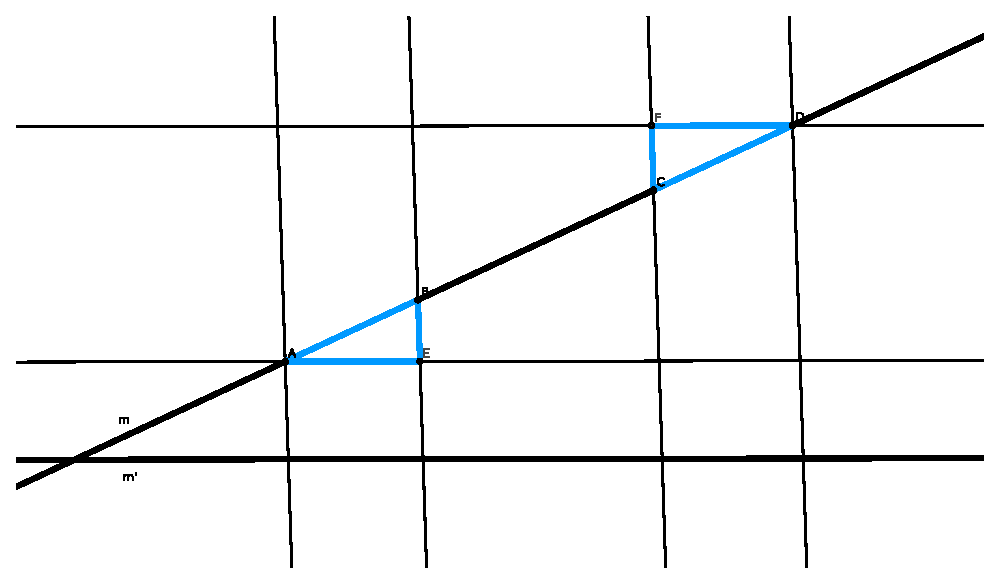
\includegraphics[scale=0.2]{semblable2.2.eps}
    \end{figure}

Cela signifie que $AE \equiv FD$, or par construction, nous savons que  les quadrilatères $AEA'B'$ et $FDC'D'$ sont des parallèlogrammes (définition des parallèlogrammes) et que $A'B' \equiv C'D'$.
\begin{figure}[H]
        \centering
        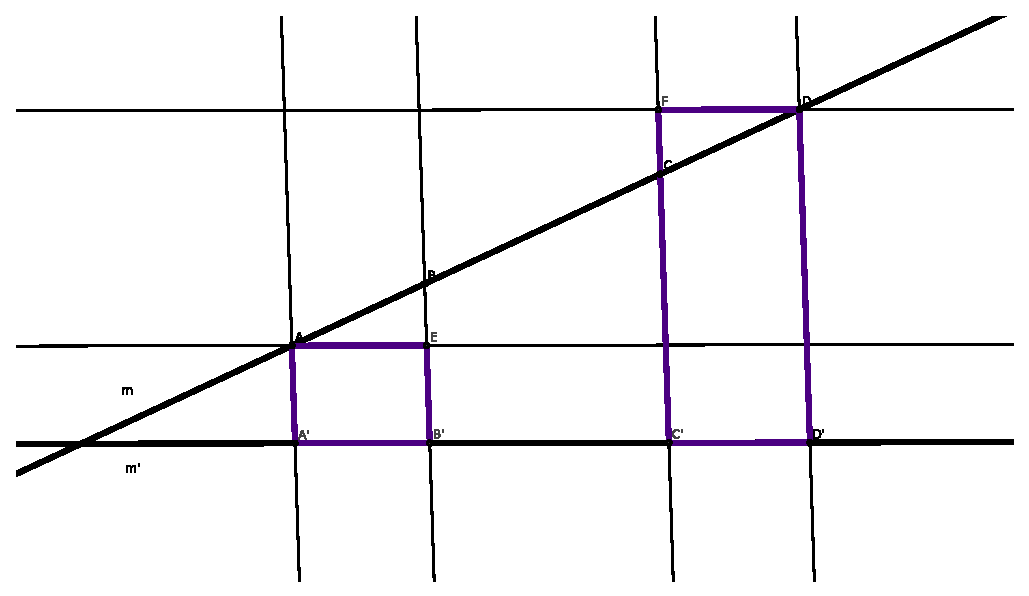
\includegraphics[scale=0.2]{semblable2.3.eps}
    \end{figure}
    
\end{proof}

\end{document}